\documentclass[11pt,a4paper]{article}

% Packages
\usepackage[utf8]{inputenc}
\usepackage[spanish, es-tabla, es-lcroman]{babel}
\usepackage{caption}
\usepackage{listings}
\usepackage{adjustbox}
\usepackage{amssymb, amsmath, amsthm}
\usepackage[margin=1in]{geometry}
\usepackage[shortlabels]{enumitem}
\usepackage{xcolor}
\usepackage{soul}
\usepackage{listings}
\usepackage{graphicx}
\usepackage{float}

% Meta
\title{Práctica 1: Eficiencia}
\author{José Antonio Álvarez Ocete}
\date{\today}

% Custom
\providecommand{\abs}[1]{\lvert#1\rvert}
\setlength\parindent{0pt}
\definecolor{Light}{gray}{.90}
\newcommand\ddfrac[2]{\frac{\displaystyle #1}{\displaystyle #2}}

% Listings
\lstset{literate=   % listings config
  {á}{{\'a}}1 {é}{{\'e}}1 {í}{{\'i}}1 {ó}{{\'o}}1 {ú}{{\'u}}1
  {Á}{{\'A}}1 {É}{{\'E}}1 {Í}{{\'I}}1 {Ó}{{\'O}}1 {Ú}{{\'U}}1
  {à}{{\`a}}1 {è}{{\`e}}1 {ì}{{\`i}}1 {ò}{{\`o}}1 {ù}{{\`u}}1
  {À}{{\`A}}1 {È}{{\'E}}1 {Ì}{{\`I}}1 {Ò}{{\`O}}1 {Ù}{{\`U}}1
  {ä}{{\"a}}1 {ë}{{\"e}}1 {ï}{{\"i}}1 {ö}{{\"o}}1 {ü}{{\"u}}1
  {Ä}{{\"A}}1 {Ë}{{\"E}}1 {Ï}{{\"I}}1 {Ö}{{\"O}}1 {Ü}{{\"U}}1
  {â}{{\^a}}1 {ê}{{\^e}}1 {î}{{\^i}}1 {ô}{{\^o}}1 {û}{{\^u}}1
  {Â}{{\^A}}1 {Ê}{{\^E}}1 {Î}{{\^I}}1 {Ô}{{\^O}}1 {Û}{{\^U}}1
  {œ}{{\oe}}1 {Œ}{{\OE}}1 {æ}{{\ae}}1 {Æ}{{\AE}}1 {ß}{{\ss}}1
  {ű}{{\H{u}}}1 {Ű}{{\H{U}}}1 {ő}{{\H{o}}}1 {Ő}{{\H{O}}}1
  {ç}{{\c c}}1 {Ç}{{\c C}}1 {ø}{{\o}}1 {å}{{\r a}}1 {Å}{{\r A}}1
  {€}{{\EUR}}1 {£}{{\pounds}}1 {ñ}{{\~{n}}}1
}

\lstset{    %listings config
  language=C++,
  belowcaptionskip=1\baselineskip,
  breaklines=true,
  frame=L,
  xleftmargin=0.1in,
  %otherkeywords={},
  showstringspaces=false,
  backgroundcolor=\color{white},
  basicstyle=\footnotesize\ttfamily,
  keywordstyle=\bfseries\color{purple!90!black},
  commentstyle=\itshape\color{gray!85!},
  identifierstyle=\color{blue!80!black},
  stringstyle=\color{green!60!black},
}

\begin{document}

\maketitle

\section{Informe de la eficiencia}

Antes de comenzar con los ejercicios voy a describir el ordenador en el que los he realizado. Adjunto un archivo \textbf{cpuinfo.txt} con la información de la CPU, con un procesador de 2 cores fisicos e Intel Core i7-5500U, 2.40GHz. La gráfica es una Nvidia GeForce 920M  y tiene una RAM de 8GB. 

En cuanto al sistema operativo, he usado Linux v16.04, el compilador es g++, la versión por defecto. No he usado opciones de compilación salvo \emph{-o}, con una única excepción en el ejercicio 6.

He adjuntado todos los códigos fuente y los scripts usados, incluyendo en este documento unicamente los fragmentos más relevantes. También he incluido todos los datos recopilados, registros  y capturas de todas las ordenes \emph{fit} de gnuplot ejecutadas y todas las gráficas.

\section{Ejercicios}

\subsection{Ejercicio 1: Ordenación de la Burbja}
El siguiente código realiza la ordenación mediante el algoritmo de la burbuja:
\begin{lstlisting}
void ordenar(int *v, int n) {
	for (int i=0; i<n-1; i++)
		for (int j=0; j<n-i-1; j++)
			if (v[j]>v[j+1]) {
				int aux = v[j];
				v[j] = v[j+1];
				v[j+1] = aux;
			}
		}
	}
}
\end{lstlisting}
Calcule la eficiencia teórica de este algoritmo. A continuación replique el experimento que se ha hecho antes (búsqueda lineal) con este nuevo código. Debe:
\begin{itemize}
	\item Crear un fichero ordenacion.cpp con el programa completo para realizar una ejecución del algoritmo.
	\item Crear un script ejecuciones\_ordenacion.csh en C-Shell que permite ejecutar varias veces el programa anterior y generar un fichero con los datos obtenidos.
	\item Usar gnuplot para dibujar los datos obtenidos en el apartado previo.
\end{itemize}
Los datos deben contener tiempos de ejecución para tamaños del vector 100, 600, 1100, ...,
30000.
Pruebe a dibujar superpuestas la función con la eficiencia teórica y la empírica. ¿Qué
sucede?

\newpage

\textbf{\underline{Solución:}}

El archivo fuente (\textbf{ordenacion.cpp}) y el script (\textbf{ejecuciones\_ordenacion.sh}) están adjuntos, así como los datos obtenidos. Representamos ahora los datos mediante gnuplot:

\begin{figure}[H]
	\centering
	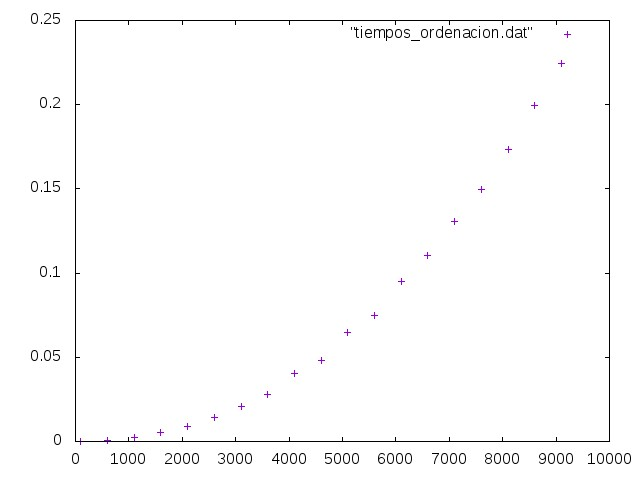
\includegraphics[width=0.8\textwidth]{Capturas_y_graficas/grafica1_1.jpg}
	\caption{Tiempos de ordenación}
\end{figure}

Aunque la eficiencia es evidentemente de orden $O(n^2)$, calculamos el polinomio completo, con sus coeficientes, para poder representarlo. Primero explicaremos de donde viene cada coeficiente y depués obtendremos el polinomio:
\begin{itemize}
	\item (for) + (comprobación, 2) + (inicialización) = 4, al entrar al primer bucle.
	\item Dentro del primer bucle, de i=0 hasta n-1:
	\begin{itemize}
		\item (comprobación, 2) + (incremento) = 3, en cada iteración del primer bucle.
		\item (for) + (comprobación, 3) + (inicialización) = 5, al entrar al segundo bucle.
		\item Dentro del segundo bucle, de j=0 hasta n-i-1:
		\begin{itemize}
			\item (comprobación, 3) + (incremento) = 4, en cada iteración del bucle.
			\item 13, interior del bucle.
		\end{itemize}
	\end{itemize}
\end{itemize}

Formalizamos matemáticamente y simplificamos:

$$4 + \sum_{i=0}^{n-1}{(3 + 5 + \sum_{j=0}^{n-i-1}{4 + 13})} $$
$$ = 4 + \sum_{i=0}^{n-1}{(8 + 17 * \sum_{j=0}^{n-i-1}{1})} $$
$$ = 4 + 8 * (n - 1) + 17 \sum_{i=0}^{n-1}{\sum_{j=0}^{n-i-1}{1}} $$
$$ = 4 + 8 * (n - 1) + 17 \sum_{i=0}^{n-1}{(n - i - 1)} $$
$$ = 4 + 8 * (n - 1) + 17 \sum_{i=0}^{n-1}{n} - \sum_{i=0}^{n-1}{i} - \sum_{i=0}^{n-1}{1}$$
$$ = 4 + 8 * (n - 1) + 17 (n*(n - 1) - n*\frac{n-1}{2} - (n-1))$$
$$ = 8.5*n^2 - 17.5*n + 13$$

Al pintar esta gráfica junto a los datos obtenidos anteriormente obtenemos el siguiente resultado:

\begin{figure}[H]
	\centering
	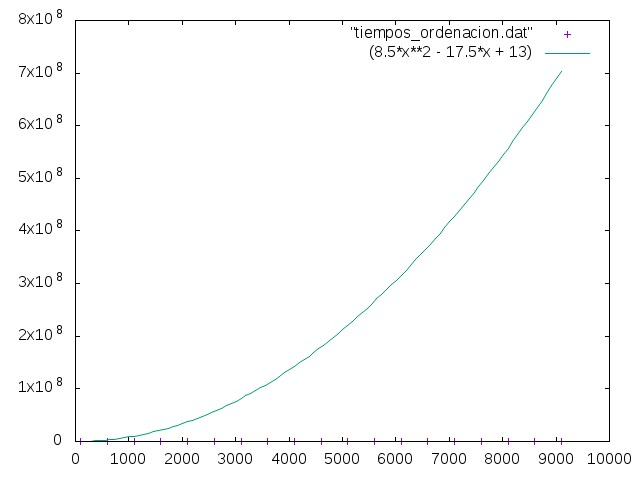
\includegraphics[width=0.8\textwidth]{Capturas_y_graficas/grafica1_2.jpg}
	\caption{Comparativa empírica - teórica 1}
\end{figure}

Como podemos ver, todos los datos se agrupan sobre el eje X. Esto se debe a que los estos valores son muchísimo más pequeños que la gráfica obtenida teóricamente. Para apreciar más o menos que ambas funciones son del mismo orden, multiplicamos la función teórica por un factor atenuante.

\begin{figure}[H]
	\centering
	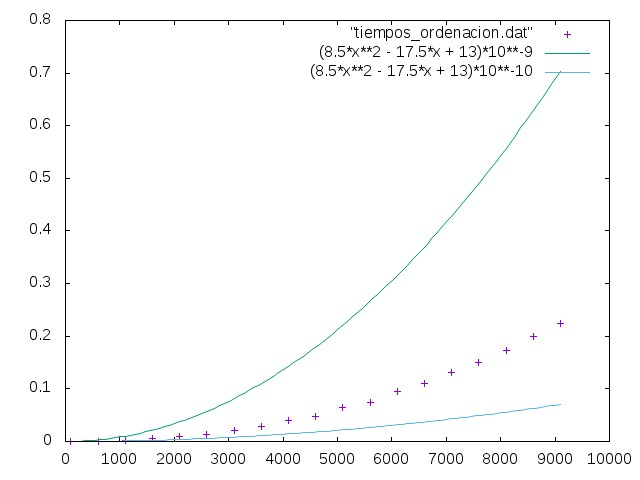
\includegraphics[width=0.8\textwidth]{Capturas_y_graficas/grafica1_3.jpg}
	\caption{Comparativa empírica - teórica 2}
\end{figure}

\subsection{Ejercicio 2: Ajuste en la ordenación de la burbuja}
Replique el experimento de ajuste por regresión a los resultados obtenidos en el ejercicio 1 que calculaba la eficiencia del algoritmo de ordenación de la burbuja. Para ello considere que f(x) es de la forma $a*x^2 + b*x + c$. \\

\newpage

\textbf{\underline{Solución:}}

Realizamos el ajuste mediante gnuplot, (el registro del ajuste está almacenado como \textbf{fit.log(2\_1)}) obteniendo los siguientes resultados:

\begin{figure}[H]
	\centering
	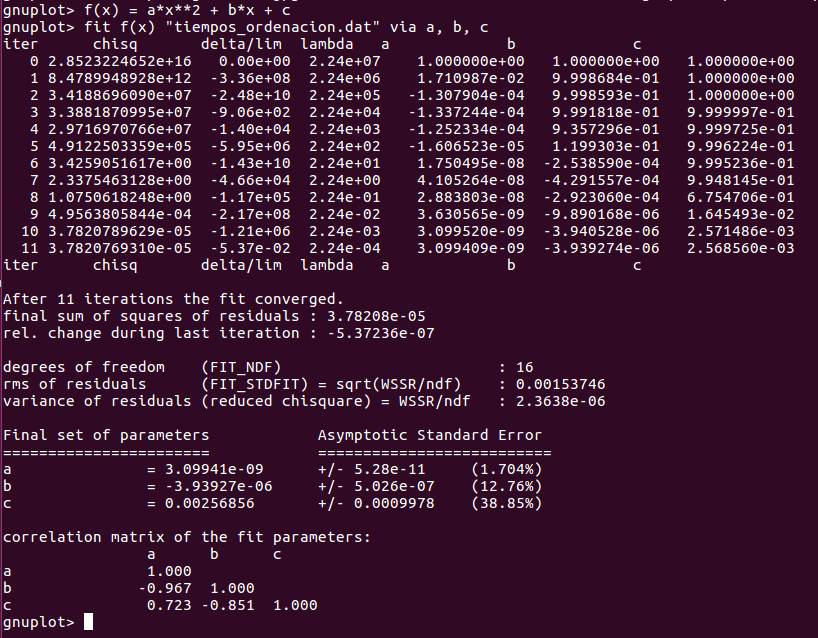
\includegraphics[width=0.8\textwidth]{Capturas_y_graficas/Ejer2_1.png}
	\caption{Ajuste empírico del ejercicio 1}
\end{figure}

Representamos ahora el ajuste obtenido frente a los datos:

\begin{figure}[H]
	\centering
	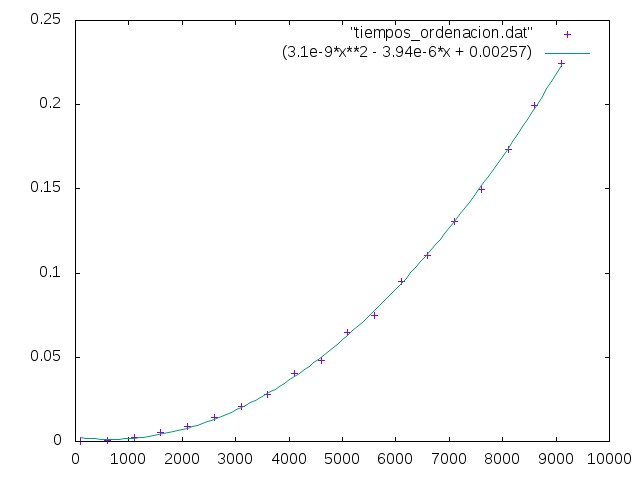
\includegraphics[width=0.8\textwidth]{Capturas_y_graficas/grafica2_1.jpg}
	\caption{Ajuste empírico frente a los datos obtenidos en el ejercicio 1}
\end{figure}

\subsection{Ejercicio 3: Problemas de precisión}
Junto con este guión se le ha suministrado un fichero ejercicio\_desc.cpp. En él se ha implementado un algoritmo. Se pide que:
\begin{itemize}
	\item Explique qué hace este algoritmo.
	\item Calcule su eficiencia teórica.
	\item Calcule su eficiencia empírica.
\end{itemize}
Si visualiza la eficiencia empírica debería notar algo anormal. Explíquelo y proponga una solución. Compruebe que su solución es correcta. Una vez resuelto el problema realice la regresión para ajustar la curva teórica a la empírica. \\

\textbf{\underline{Solución:}}

Este algoritmo implementa una búsquedad binaria. Cabe destacar que este algoritmo se aplica sobre un vector ordenado, condición que en este caso no estamos cumpliendo. Obviamente no nos interesa encontrar el elemento (de hecho forzamos que no pueda encontrarse) sino estudiar la eficiencia en el peor caso posible: que el elemento no se halle en el vector.

En cuanto al estudio teórico, es bastante sencillo: la eficiencia es del orden $O(log(n))$. Esto se debe a que reducimos el vector en el que buscamos a la mitad en cada iteración, provocando una progresión de orden logarítmico.

Tomamos muestras de tiempo y las representamos:

\begin{figure}[H]
	\centering
	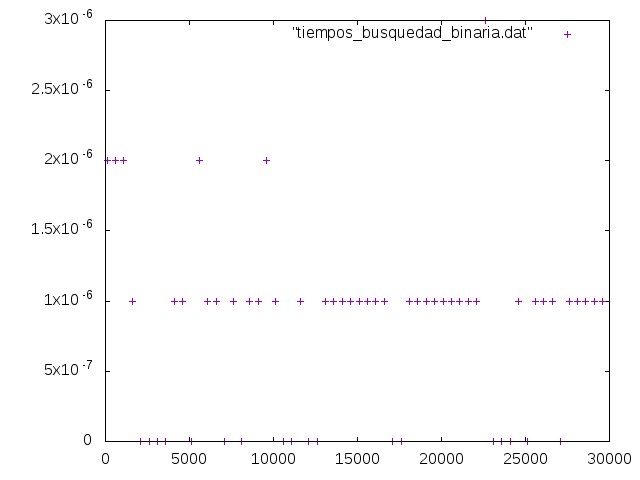
\includegraphics[width=0.8\textwidth]{Capturas_y_graficas/grafica3_1.jpg}
	\caption{Tiempos de búsquedad binaria 1}
\end{figure}

Evidentemente hemos cometido un error: la función \emph{clock()} tiene dificultades para medir tiempos muy pequeños, como es el caso de este algoritmo de eficiencia logarítmica. Para resolver esto realizamos numerosas ejecuciones (denotémoslo por \emph{MAX}), medimos el tiempo del total y dividimos por \emph{MAX}. Adjunto un fragmento del archivo \textbf{ejercicio\_desc.cpp} modificado (el cual también va adjunto):

\begin{lstlisting}
  const long int MAX=10000;
  double timedif;
  tini=clock();
  for (int i=0; i<MAX; i++) {
    operacion(v,tam,tam+1,0,tam-1);
  }
  tfin=clock();
  timedif = (tfin-tini)/(double)CLOCKS_PER_SEC;
  timedif /= MAX;
\end{lstlisting}

Utilizando esta implementación repetimos el proceso de muestreo:

\begin{figure}[H]
	\centering
	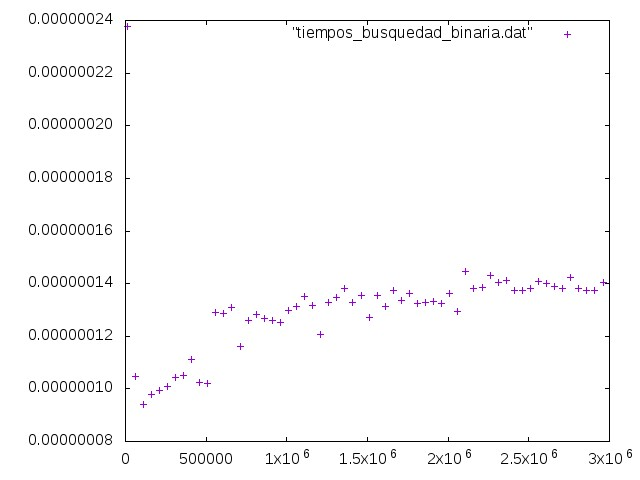
\includegraphics[width=0.8\textwidth]{Capturas_y_graficas/grafica3_2.jpg}
	\caption{Tiempos de búsquedad binaria 2}
\end{figure}

Por último realizamos un ajuste conforme a los datos obtenidos utilizando la función $f(x) = a*log(b*x) + c$:

\begin{figure}[H]
	\centering
	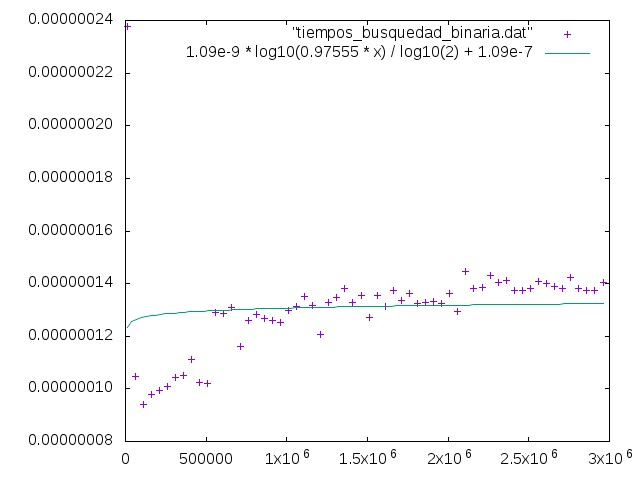
\includegraphics[width=0.8\textwidth]{Capturas_y_graficas/grafica3_3.jpg}
	\caption{Tiempos de búsquedad binaria y ajuste.}
\end{figure}

\subsection{Ejercicio 4: Mejor y peor caso}
Retome el ejercicio de ordenación mediante el algoritmo de la burbuja. Debe modificar el código que genera los datos de entrada para situarnos en dos escenarios diferentes:
\begin{itemize}
	\item El mejor caso posible. Para este algoritmo, si la entrada es un vector que ya está ordenado el tiempo de cómputo es menor ya que no tiene que intercambiar ningún elemento.
	\item El peor caso posible. Si la entrada es un vector ordenado en orden inverso estaremos en la peor situación posible ya que en cada iteración del bucle interno hay que hacer un intercambio.
\end{itemize}
Calcule la eficiencia empírica en ambos escenarios y compárela con el resultado del ejercicio 1.\\

\textbf{\underline{Solución:}}

El mejor caso posible es aquel en el que el vector ya está ordenado. El peor caso es aquel en el que el vector está ordenado de forma inversa (de mayor a menor. Ahora pasamos sendos vectores creados de esta forma al algoritmo de ordenación y tomamos tiempos. Adjuntamos aquí el fragmento del código en el que se crean los vectores (\emph{mejor} es un parámetro de entrada al programa). El código completo se encuentra en el archivo \textbf{ordenacionMejorPeor.cpp}.

\begin{lstlisting}
int *v=new int[tam];
  if (mejor) {
    for (int i=0; i<tam; i++) {
      v[i] = i;
    }
  } else {
    for (int i=0; i<tam; i++) {
      v[i] = tam - i;
    }
  }
\end{lstlisting}

Representamos los datos obtenidos:

\begin{figure}[H]
	\centering
	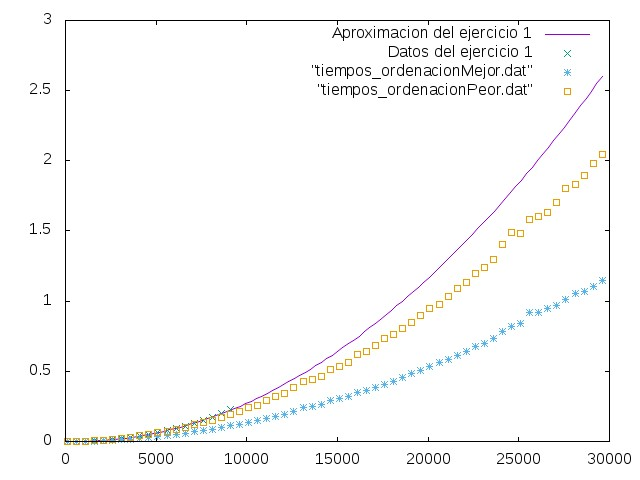
\includegraphics[width=0.8\textwidth]{Capturas_y_graficas/grafica4_1.jpg}
	\caption{Mejor, peor y caso promedio de ordenación por burbuja}
\end{figure}

Como podemos observar en la gráfica, el mejor caso es el que menos tiempo requiere. Sin embargo, el peor caso está aparentemente mal realizado: según esta gráfica el caso aleatorio requiere más tiempo que el peor caso posible. No he encontrado una explicación clara para este hecho. Si me he asegurado, por otro lado, de asegurarme de que la creación del vector, la toma de datos y el uso de \emph{gnuplot} están bien realizados. Por último, utilizamos de nuevo la función \emph{fit} de gnuplot sobre estos datos para obtener sendas aproximaciones de ambos:

\begin{figure}[H]
	\centering
	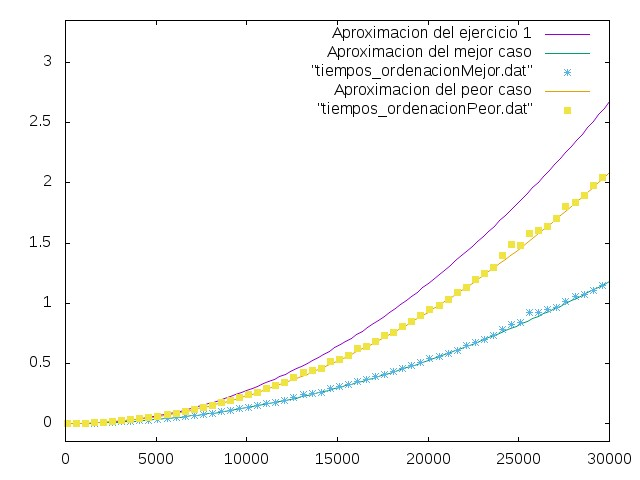
\includegraphics[width=0.8\textwidth]{Capturas_y_graficas/grafica4_2.jpg}
	\caption{Aproximaciones del mejor, peor y caso promedio.}
\end{figure}

\subsection{Ejercicio 5: Dependencia de la implementación}
Considere esta otra implementación del algoritmo de la burbuja:
void ordenar(int *v, int n) {
bool cambio=true;
\begin{lstlisting}
void ordenar(int *v, int n) {
	for (int i=0; i<n-1 && cambio; i++) {
		cambio=false;
		for (int j=0; j<n-i-1; j++) {
			if (v[j]>v[j+1]) {
				cambio=true;
				int aux = v[j];
				v[j] = v[j+1];
				v[j+1] = aux;
			}
		}
	}
}
\end{lstlisting}
En ella se ha introducido una variable que permite saber si, en una de las iteraciones del bucle externo no se ha modificado el vector. Si esto ocurre significa que ya está ordenado y no hay que continuar.
Considere ahora la situación del mejor caso posible en la que el vector de entrada ya está ordenado. ¿Cuál sería la eficiencia teórica en ese mejor caso? Muestre la gráfica con la eficiencia empírica y compruebe si se ajusta a la previsión.\\

\textbf{\underline{Solución:}}

Ante esta nueva implementación y con el vector ya ordenado, el algoritmo se reduce a una iteración del bucle (recorrerlo y comprobar que esta ordenado). Es decir, su eficiencia es del orden \emph{O(n)}. Evidentemente no tiene nada que ver con la implementación anterior:

\begin{figure}[H]
	\centering
	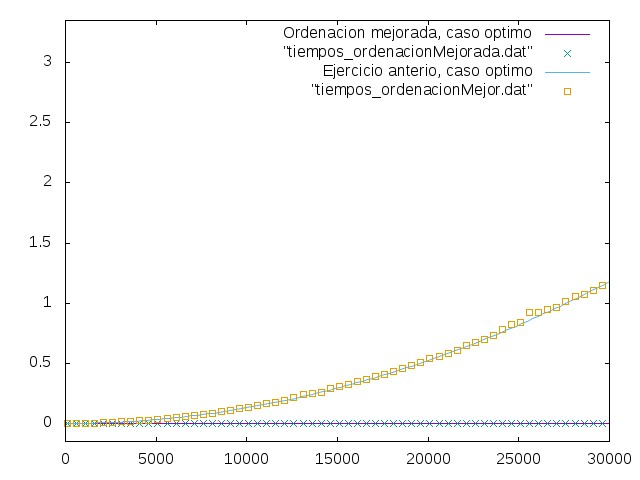
\includegraphics[width=0.8\textwidth]{Capturas_y_graficas/grafica5_1.jpg}
	\caption{Dependencia de la implementación.}
\end{figure}

\subsection{Ejercicio 6: Influencia del proceso de compilación}
Retome el ejercicio de ordenación mediante el algoritmo de la burbuja. Ahora replique dicho ejercicio pero previamente deberá compilar el programa indicándole al compilador que optimice el código. Esto se consigue así.
\[ g++ -O3 ordenacion.cpp -o ordenacion\_optimizado\] 
Compare las curvas de eficiencia empírica para ver cómo mejora esto la eficiencia del programa. \\

\textbf{\underline{Solución:}}

Compilamos de la forma indicada, ejecutamos para obtener los datos y representamos el resultado frente a los datos del ejercicio anterior:

\begin{figure}[H]
	\centering
	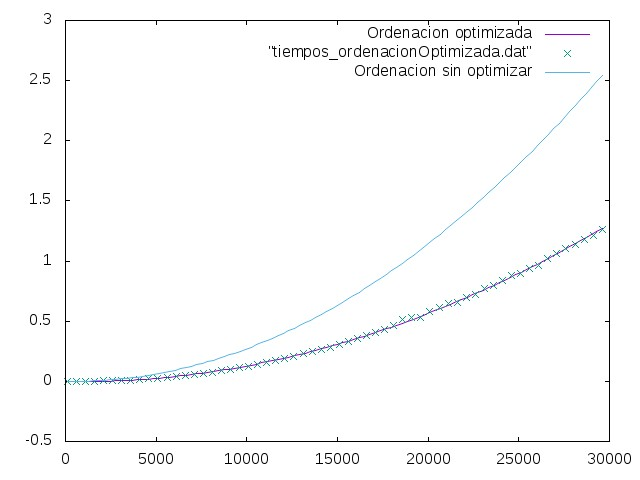
\includegraphics[width=0.8\textwidth]{Capturas_y_graficas/grafica6_1.jpg}
	\caption{Influencia del proceso de compilación.}
\end{figure}

Nota: Este es el único ejercicio que no lleva asociado ningún archivo de código fuente (se ha compilado a partir del original, como indica el enunciado) pero si que lleva asociado un script, \textbf{ejecuciones\_ordenacionOptimizada.sh}, para mayor comodidad.

\subsection{Ejercicio 7: Multiplicación matricial}
Implemente un programa que realice la multiplicación de dos matrices bidimensionales. Realice un análisis completo de la eficiencia tal y como ha hecho en ejercicios anteriores de este guión. \\

\textbf{\underline{Solución:}}

Adjuntamos aquí el fragmento de \textbf{MM.cpp} que implementa la multiplicación como tal:

\begin{lstlisting}
void mult(int **m1, int **m2, int **m3, int tam) {
  int result;
  for (int i=0; i<tam; i++) {
    for (int j=0; j<tam; j++) {
      result = 0;
      for (int k=0; k<tam; k++) {
        result += m1[i][k] * m2[k][j];
      }
      m3[i][j] = result;
    }
  }
}
\end{lstlisting}

El estudio teórico de la eficiencia de este código es sencillo: tenemos tres bucles anidados, de $i,j,k = 0$ hasta \emph{tam}, el tamaño de las matrices. Llamando $n = tam$, la eficiencia de la multiplicación de matrices implementada en este código es de $O(n^3)$.

Repetimos el procedimiento seguido en los otros ejercicios ajustando los datos a una función de la forma $f(x) = a*x^3 + b*x^2 + c*x + d$.

\begin{figure}[H]
	\centering
	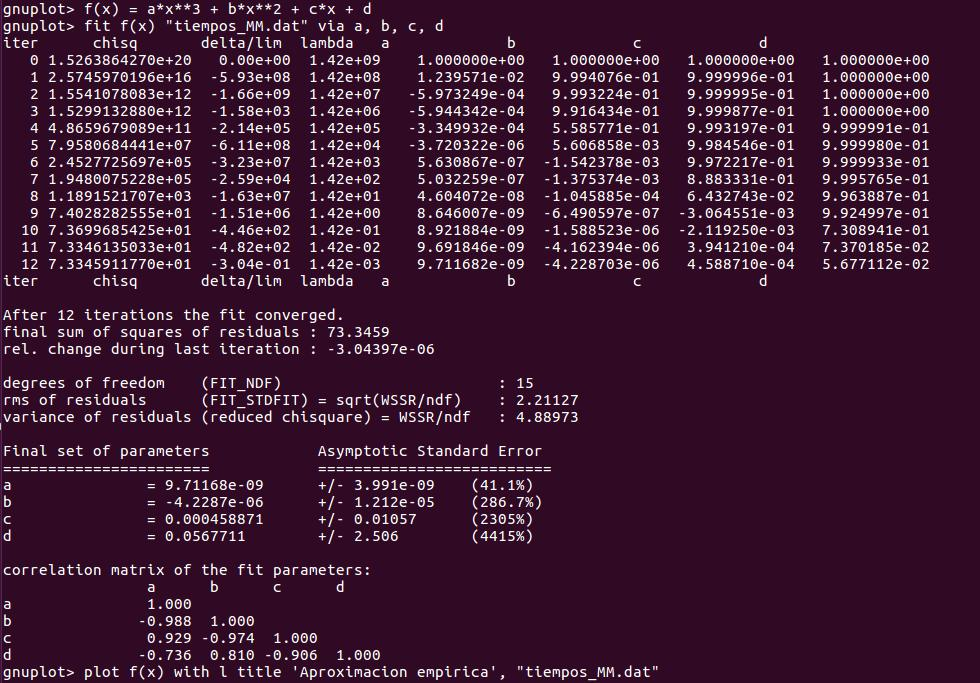
\includegraphics[width=0.8\textwidth]{Capturas_y_graficas/Ejer7_1.png}
	\caption{Ajuste de la eficiencia empírica de la multipliación de matrices.}
\end{figure}

\newpage

Por último, representamos los datos:

\begin{figure}[H]
	\centering
	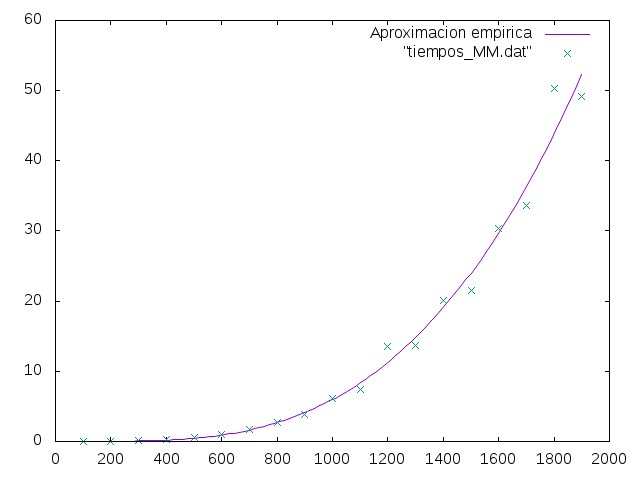
\includegraphics[width=0.8\textwidth]{Capturas_y_graficas/grafica7_1.jpg}
	\caption{Eficiencia de la multiplicación de matrices.}
\end{figure}

\subsection{Ejercicio 8: Ordenación por Mezcla}
Estudie el código del algoritmo recursivo disponible en el fichero mergesort.cpp. En él, seintegran dos algoritmos de ordenación: inserción y mezcla (o mergesort). El parámetro UMBRAL\_MS condiciona el tamaño mínimo del vector para utilizar el algoritmo de inserción en vez de seguir aplicando de forma recursiva el mergesort. Como ya habrá estudiado, la eficiencia teórica del mergesort es n log(n). Realice un análisis de la eficiencia empírica y haga el ajuste de ambas curvas. Incluya también, para este caso, un pequeño estudio de cómo afecta el parámetro UMBRAL\_MS a la eficiencia del algoritmo .Para ello, pruebe distintos valores del mismo y analice los resultados obtenidos. \\

\textbf{\underline{Solución:}}

Tomamos los datos y ajustamos la función $f(x) = a*x*log(x) + b*x + c$. (Aunque en primer lugar intenté ajustar los datos a $f(x) = a*x*log(b*x) + c*x + d$, los resultados dejaban mucho que desear).

\begin{figure}[H]
	\centering
	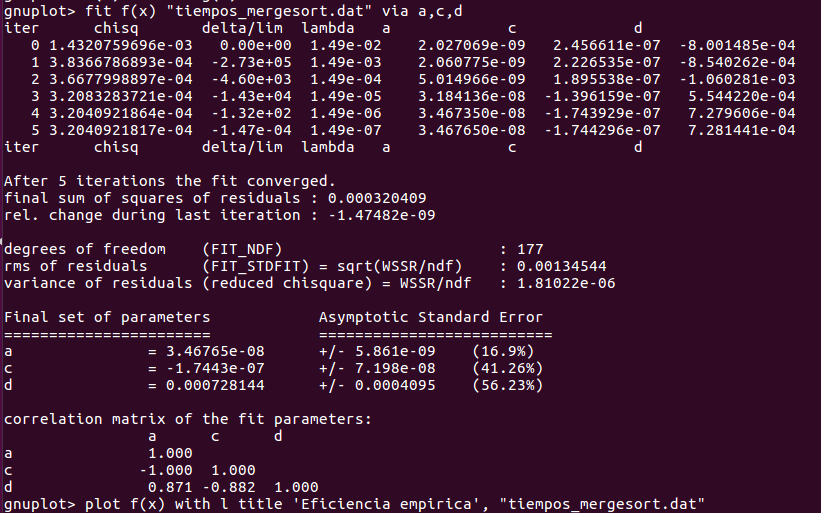
\includegraphics[width=0.8\textwidth]{Capturas_y_graficas/Ejer8_1.png}
	\caption{Influencia del proceso de compilación.}
\end{figure}

Nota: Aunque en esta imagen no se aprecia la forma de f(x) (me equivoqué al tomar la captura), podemos verlo en el archivo \textbf{fit.log(8\_1)}:

\begin{verbatim}
Tue Sep 26 09:40:05 2017

FIT:    data read from "tiempos_mergesort.dat"
        format = z
        x range restricted to [-120000. : 180000.]
        #datapoints = 180
        residuals are weighted equally (unit weight)

function used for fitting: f(x)
f(x) = a*x*log(x) + c*x + d
fitted parameters initialized with current variable values

[...]

Final set of parameters            Asymptotic Standard Error
=======================            ==========================
a               = 3.46765e-08      +/- 5.861e-09    (16.9%)
c               = -1.7443e-07      +/- 7.198e-08    (41.26%)
d               = 0.000728144      +/- 0.0004095    (56.23%)

\end{verbatim}

Vemos el resultado en la siguiente imagen:

\begin{figure}[H]
	\centering
	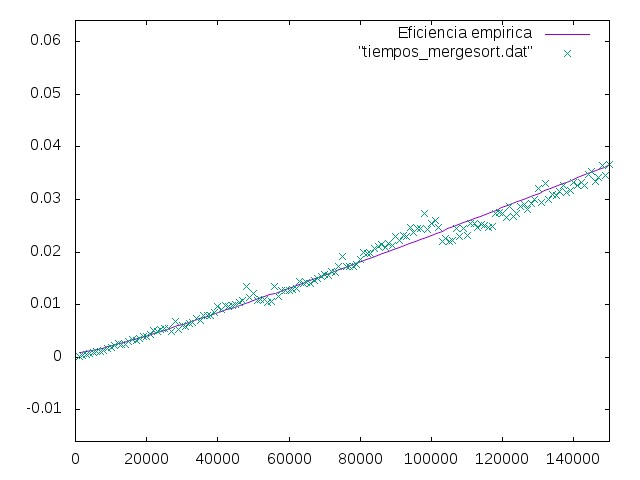
\includegraphics[width=0.8\textwidth]{Capturas_y_graficas/grafica8_1.jpg}
	\caption{Eficiencia del algoritmo Mergesort}
\end{figure}

Veamos ahora como afecta el parámetro \textbf{UMBRAL\_MS} a la eficiencia dándole distintos valores. He realizado dos estudios del algoritmo además del explicado arriba: uno para $UMBRAL\_MS = 10$ (umbral bajo) y otro para $UMBRAL\_MS = 1000$ (umbral alto). 

\begin{figure}[H]
	\centering
	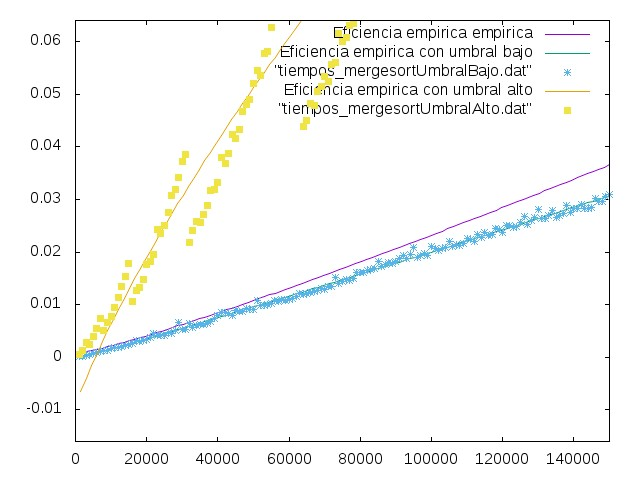
\includegraphics[width=0.8\textwidth]{Capturas_y_graficas/grafica8_2.jpg}
	\caption{Influencia del parámetro \textbf{UMBRAL\_MS}.}
\end{figure}

\newpage

Vemos como para valor alto el tiempo se dispara, ya que estamos aplicando inserción más que mergesort, mientras la eficiencia aumenta ligeramente para un valor bajo del parámetro. Evidentemente esto se debe a que aplicamos mergesort a un mayor porcentaje del vector. Sin embargo esto produce un uso extra de la pila del programa ya que supone un mayor número de llamadas recursivas. 

\end{document}